% Shared float (common/make_floats.py). Figure: figures/cnn_first_layer.pdf
\begin{figure}[htbp]
\centering
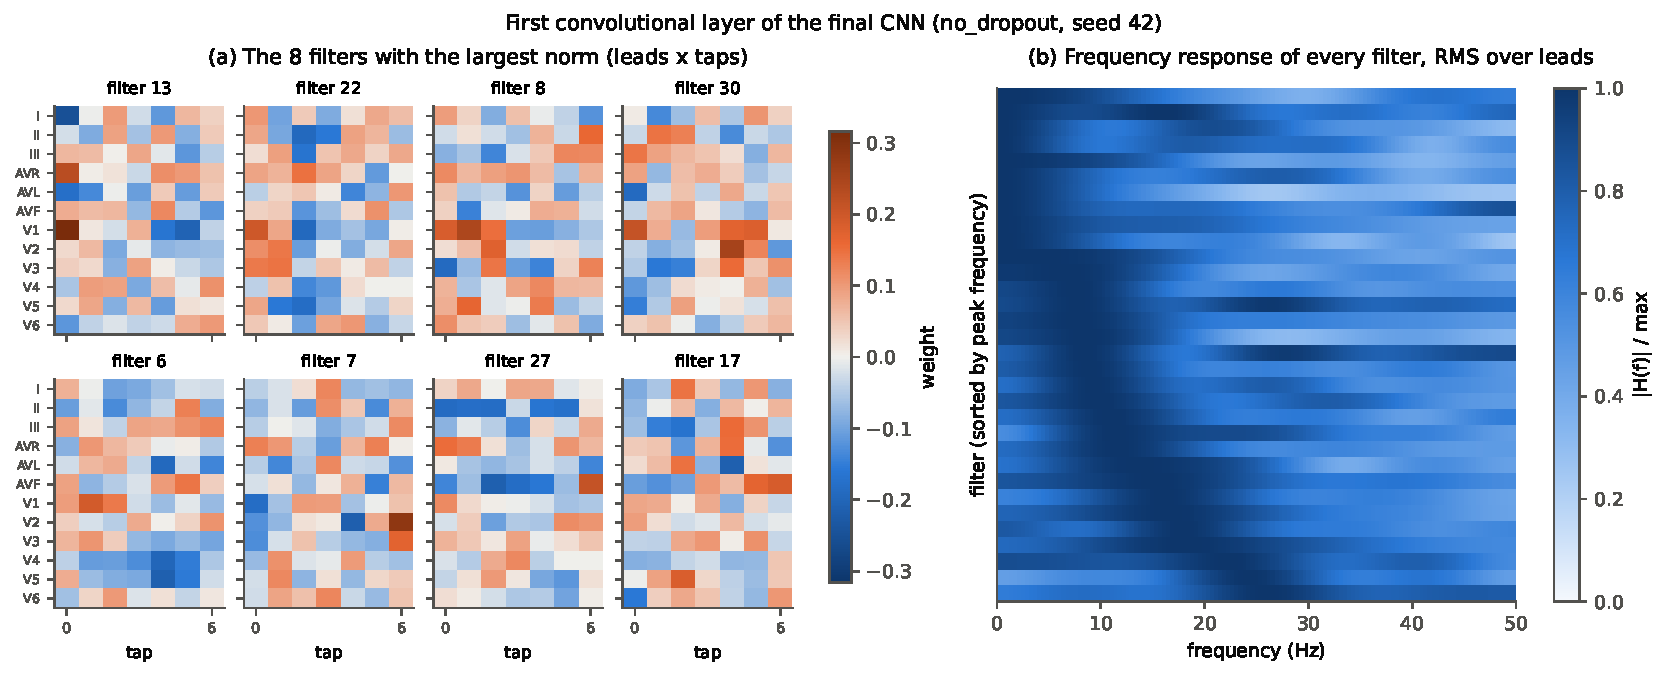
\includegraphics[width=\textwidth,height=0.42\textheight,keepaspectratio]{figures/cnn_first_layer.pdf}
\caption[1D CNN: first-layer filters]{First convolutional layer of the final CNN (\texttt{no\_dropout}, seed 42). (a) The eight filters with the largest norm (12 leads $\times$ 7 taps). (b) Frequency response of every filter (RMS over leads, normalised), sorted by peak frequency.}
\label{fig:cnn_first_layer}
\end{figure}
